\documentclass[sigconf,nonacm,10pt]{acmart}
\settopmatter{printacmref=false, printccs=false, printfolios=true}
\setcopyright{none}
\renewcommand\footnotetextcopyrightpermission[1]{}

\usepackage{graphicx}
\usepackage{url}

\newcommand{\Q}[2]{\textbf{Q#1: #2.}\;}

\title{Reproducing KLEE's Coverage Results on GNU Coreutils}
\subtitle{CSE 231: Advanced Operating Systems (Spring 2026), Prof.\ Andrea Quinn}

\author{Ethan Sifferman}
\affiliation{%
  \institution{University of California, Santa Cruz}
}
\email{sifferman@ucsc.edu}
\renewcommand{\shortauthors}{Sifferman}

\begin{document}

\begin{abstract}
I reproduced Cadar's Table~2 and Figure~5 from the OSDI'08 KLEE
paper using the official \texttt{klee/klee:3.1} Docker image,
running KLEE on 98 Coreutils 6.11 utilities for 60~min per tool.
I measured 69.95\% overall (aggregate) line-coverage (paper: 84.5\%) and
85.25\% per-tool median (paper: 94.7\%). The shape of the per-tool
curve closely matches the paper; the level gap is explained by
parallel-execution contention and a \texttt{libgcov}
crash-corruption issue I identified. I also applied KLEE to
\texttt{tinyexpr}, a small expression-parser library not covered
by the paper, achieving 63\% line-coverage and 70\% branch-coverage in 60 minutes.
Code and reproduction scripts:
\url{https://github.com/sifferman/klee-runner}.
\end{abstract}

\maketitle

\section{The Paper}

\Q{1}{Summary} \textsc{Klee}~\cite{cadar2008klee} is a
\emph{symbolic execution} engine: instead of running a program on
concrete inputs, it runs the program on placeholder
(``symbolic'') inputs, forks at every input-dependent branch, and
uses an SMT solver to derive a concrete input that drives each
reachable path. \textsc{Klee} applies this to C programs compiled
to LLVM bitcode (clang's intermediate representation). The paper
claims this achieves high line-coverage on GNU Coreutils without
per-tool specifications.

\Q{2}{Hypothesis} Symbolic execution can automatically generate
high-coverage tests on complex, environmentally-intensive
real-world programs without per-program manual modeling.

\Q{3}{Original setup} Each of 89 Coreutils 6.10 utilities was
compiled to LLVM bitcode and run under \textsc{Klee} for at most
60~min on a 2008-era machine, sequentially. Symbolic input: up to
three argv strings, two 8-byte files, 8 bytes of \texttt{stdin}.
Each tool ran twice: once normally, and once with
\texttt{--max-fail 1}, which makes \textsc{Klee} additionally
explore paths where one POSIX system call returns an error so the
tool's error-handling code is exercised. The two runs' tests were
replayed through a \texttt{gcov}-instrumented native build.

\Q{4}{Original results and support} Cadar's Table~2 reports 84.5\% Base+Fail
overall (aggregate) line-coverage (covered lines divided by total lines
summed across tools), 94.7\% per-tool median, 90.9\% mean, with
16/89 tools at 100\% and 56/89 at $\geq$90\%. The Base-only
overall is 79.9\%. These support the hypothesis.

\section{My Setup}

\Q{5}{How my setup differs} I use the official
\texttt{klee/klee:3.1} Docker image (KLEE~3.1, LLVM~13, STP, Z3,
\texttt{klee-uclibc}), provided by the autors, and Coreutils~6.11 (one
dot release later than the paper). The KLEE flag set matches
Cadar's Section~5.2, with the symbolic argument grammar from
the modern KLEE Coreutils tutorial. Three deliberate deviations:
\emph{(a)} parallelism, the paper ran sequentially while I ran
10--24 KLEE instances concurrently (each
capped at 1~GB, sharing solver subprocesses and memory bandwidth);
\emph{(b)} version, pre-release 2008 KLEE vs.\ mine at 3.1;
\emph{(c)} tool count, my build produces 98 utilities vs.\ the
paper's 89.

\section{KLEE in Practice}

\textbf{Output files.} Per tool, \textsc{Klee} writes
\texttt{testNNNNNN.\{ktest, cov, cvc\}}: \texttt{.ktest} is a
binary record of the concrete inputs (argv, files, stdin) that
drives that path, replayable on the gcov binary via
\texttt{klee-replay}; \texttt{.cov} gives that test's
line-coverage delta; \texttt{.cvc} captures the path's SMT
constraints.

\textbf{Bug types.} \textsc{Klee} flags universal-error
operations: out-of-bounds memory access, null dereferences, double
frees, division by zero, overflow checks, and programmer-written
\texttt{assert()}/\texttt{abort()}. Functional-correctness errors
need an ``oracle'' and are out of scope.

\section{Results}

\Q{6}{My results vs.\ paper's} Figure~\ref{fig:figure5} reproduces
Cadar's Figure~5: per-tool coverage sorted ascending,
two-tone bars showing Base coverage (gray, in front) and Base+Fail
(black, behind), with horizontal lines for Cadar's Table~2
statistics (dashed) and mine (solid).

\begin{figure*}[t]
  \centering
  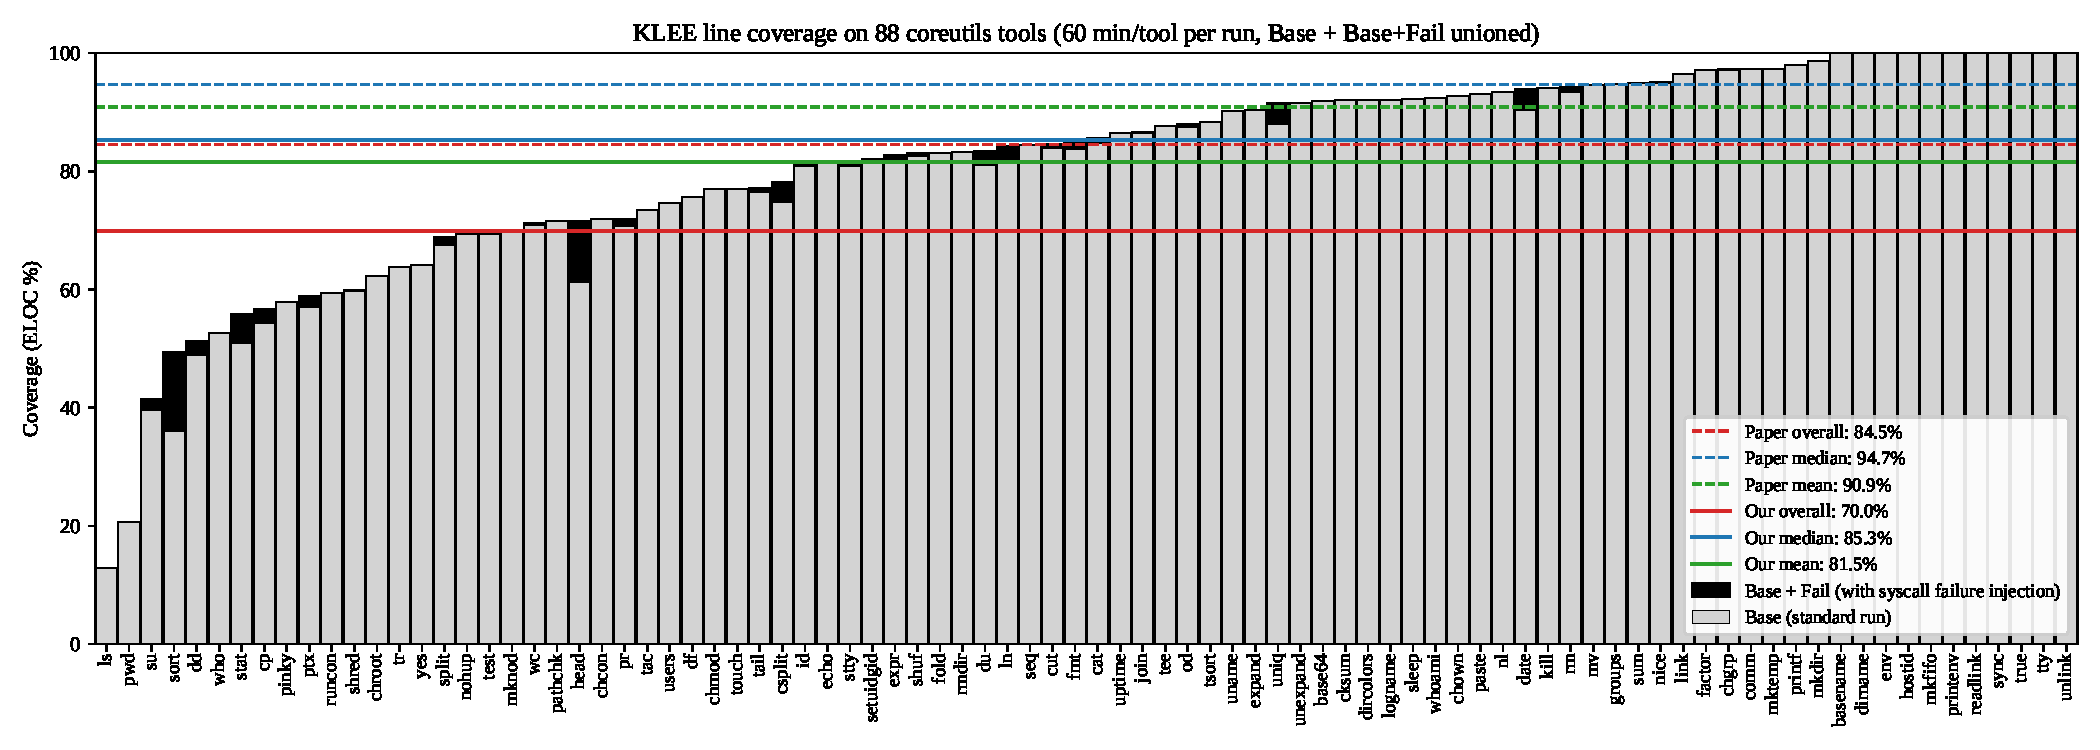
\includegraphics[width=\textwidth]{figure5_recreation.pdf}
  \par\vspace{0.6em}
  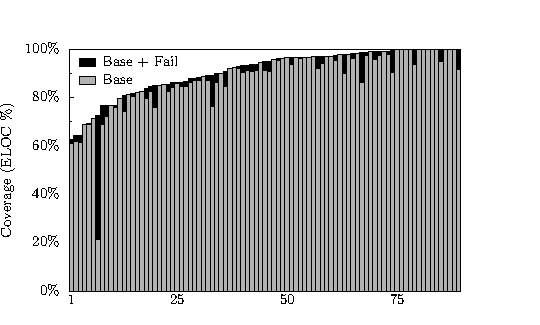
\includegraphics[width=0.45\textwidth]{figure5_cadar.pdf}
  \caption{Recreation of Cadar's Figure~5. Top: my run on 88
  Coreutils utilities. Bottom: the original. Black bars are
  Base+Fail coverage; gray bars (in front) are Base only, so
  visible black above each gray bar is the gain from
  \texttt{--max-fail 1}. Dashed lines: Cadar's Table~2 stats.
  Solid: mine. Red is overall, blue is per-tool median, green is
  per-tool mean.}
  \label{fig:figure5}
\end{figure*}

\textbf{Headline numbers (Base+Fail):} 69.95\% overall, 85.25\%
median, 81.49\% mean, 11/88 at 100\%, 36/88 at $\geq$90\%;
Base-only overall is 68.21\%. Paper: 84.5\%, 94.7\%, 90.9\%,
16/89, 56/89, 79.9\%. The curve shape matches closely: long lower
tail (\texttt{ls}, \texttt{pwd}, \texttt{sort}, \texttt{su},
\texttt{dd}), middle plateau, 100\%-cluster on the right. The
paper calls out \texttt{pwd} as its worst tool at 21.2\% Base; I
measured 20.5\%, a near-exact match.

\textbf{Why my numbers fall short.} \emph{(1) Parallelism tax}
(largest): constraint solving dominates KLEE's runtime, and
10-way contention reduces effective CPU-minutes per run; a
sequential rerun would cost $\sim$98 CPU-hours, which I did not
have time for. \emph{(2) Measurement-script gaps}: the SHA-family
binaries actually compile from \texttt{md5sum.c} via preprocessor
flags, and \texttt{dir}/\texttt{ginstall} likewise come from
\texttt{ls.c}/\texttt{install.c}. My script greps gcov's output
for the exact filename and finds nothing, so $\sim$10 utilities
drop out of my overall measurement. \emph{(3) Paper's per-tool tuning}:
the authors increased argument size for eight tools after
consulting \texttt{man} pages; I use a single fixed grammar.

\section{Coreutils Build Difficulties}

\textbf{\texttt{glibc} portability.} Coreutils 6.11 fails to
compile on modern \texttt{glibc} because its bundled gnulib reaches
into private header internals. One upstream patch and a one-line
fix in \texttt{src/sort.c} make it build cleanly.

\textbf{The \texttt{mv} \texttt{libgcov} bug.} For \texttt{mv}, my
Base+Fail measurement gave 85.71\%, lower than Base-alone's
94.51\%, which is mathematically impossible: the combined run
should have included all of Base's tests at minimum. Investigation showed
that one \texttt{--max-fail 1} test crashed \texttt{mv} via
\texttt{abort()}; \texttt{libgcov}'s hook that updates the shared
\texttt{.gcda} coverage file runs only partially on a crash,
leaving the file unparseable. The next \texttt{klee-replay} reads
it as zero, restarting the cumulative count and erasing prior
coverage. Since combined must dominate Base by construction, my
plotting script displays \texttt{max(base, combined)} per tool.
This fix triggered exactly once (for \texttt{mv}), placing it back
in the high-coverage cluster.

\section{Extension: KLEE on \texttt{tinyexpr}}

The paper covers Coreutils, BusyBox, MINIX, and HiStar but no
parser libraries. I applied \textsc{Klee} to
\texttt{tinyexpr}~\cite{tinyexpr}, an 821-LOC recursive-descent
expression evaluator, via a 5-line harness calling
\texttt{te\_compile()} (parse-only; \textsc{Klee} cannot
symbolically execute floating-point). After 60~min,
\textsc{Klee} generated 37 test cases, completed 934 paths
(another 24,803 paths were partially explored when the timer
expired), and the replayed tests covered 63.01\% of 365 source
lines and 69.89\% of 269 branches in \texttt{tinyexpr.c}.
\textsc{Klee} became solver-bound (TSolver $>$~99\%) within
minutes: tinyexpr's tokenizer calls uclibc's \texttt{strtod} on
every digit, and \texttt{strtod} has many branches. The methodology
ports cleanly, but constraint explosion is more pronounced than on
the paper's CLI tools, suggesting parsers are a harder target for
symbolic execution than the command-line utilities the paper
evaluated.

\section{Discussion}

\Q{7}{Does the hypothesis still hold} Yes. My
per-tool curve shape matches the paper's. 88\% of measured
Coreutils tools exceed 60\% coverage, 41\% exceed 90\%, and the
median is 85.25\%. That is below the paper's 94.7\% but
unambiguously ``high coverage, unassisted, on real code,'' which
is the hypothesis. The shortfall is explained by factors likely
unrelated to the algorithm: parallelism contention and measurement
artifacts. The
\texttt{tinyexpr} extension reinforces this: the same methodology
ported to a parser library outside the paper's chosen targets and
still produced respectable coverage (63\% lines, 70\% branches),
even when the constraint solver became the bottleneck.

\bibliographystyle{ACM-Reference-Format}
\bibliography{refs}

\end{document}
